% Figure 2 (Section 3.2): the shared-noise estimate of the self-rotation likelihood ratio. Image: CIFAR-10 test 3535 (a dog), noised with sigma = 0.3 for visibility, T = R90 (figs/sh_*.pdf: paper/gen/mk_thumbs.py). The values in the caption are the macros sh* of numbers.tex (the coarsest atom of the rule, (R90, sigma_7)).
\begin{figure*}[t]\centering
\begin{adjustbox}{max width=\textwidth}
\begin{tikzpicture}[font=\footnotesize,>={Stealth[length=1.6mm]},
  img/.style={inner sep=0pt,draw=black!40},
  box/.style={draw,rounded corners=2pt,align=center,inner sep=2.5pt,minimum height=7mm,fill=white},
  res/.style={draw,rounded corners=2pt,align=center,inner sep=2.5pt,minimum height=7mm,fill=firstblue!45},
  key/.style={draw,rounded corners=2pt,align=left,inner sep=4pt,text width=49mm,minimum height=22mm,font=\footnotesize,fill=white},
  lab/.style={font=\scriptsize,align=center},
  stg/.style={font=\scriptsize\bfseries,fill=white,inner sep=1.5pt}]
% ================================================================ the computation at one noise scale sigma
% inputs
\node[img] (x) at (0,0.75) {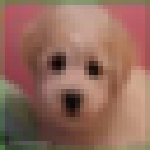
\includegraphics[width=1.1cm]{figs/sh_x.pdf}};
\node[lab,below=1pt of x] {画像 $\vec{x}$};
\node[img] (e) at (0,-1.45) {
\includegraphics[width=1.1cm]{figs/sh_eps.pdf}};
\node[lab,below=1pt of e] {ノイズ $\veps\sim\mathcal{N}(\vec{0},\mI)$};
\node[img] (xs) at (2.9,-0.35) {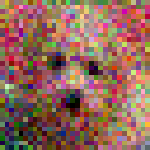
\includegraphics[width=1.1cm]{figs/sh_xs.pdf}};
\node[lab,below=1pt of xs] {$\vec{x}_\sigma=\vec{x}+\sigma\veps$};
\draw[->] (x.east) -- ($(xs.west)+(0,0.3)$);
\draw[->] (e.east) -- ($(xs.west)+(0,-0.3)$);
% upright branch
\node[box] (d1) at (6.6,0.75) {ノイズ除去器\\$\epsth(\cdot,\sigma)$};
\draw[->] ($(xs.east)+(0,0.3)$) -- ++(0.45,0) |- node[pos=0.72,above,lab] {そのまま} (d1.west);
\node[box] (b) at (10.0,0.75) {正立の予測ノイズ\\$\vec{b}=\epsth(\vec{x}_\sigma)$};
\draw[->] (d1) -- (b);
% rotated branch
\node[img] (txs) at (6.6,-1.95) {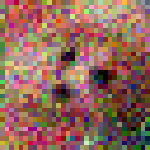
\includegraphics[width=1.1cm]{figs/sh_txs.pdf}};
\node[lab,below=1pt of txs] {$\mT\vec{x}_\sigma=\mT\vec{x}+\sigma \mT\veps$};
\draw[->] ($(xs.east)+(0,-0.3)$) -- ++(0.45,0) |- node[pos=0.74,below,lab] {回転 $\mT=\Rot{90}$} (txs.west);
\node[box] (d2) at (9.7,-1.95) {ノイズ除去器\\$\epsth(\cdot,\sigma)$};
\draw[->] (txs) -- (d2);
\node[box] (a) at (14.2,-1.95) {逆回転した予測ノイズ\\$\vec{a}=\mT^{-1}\epsth(\mT\vec{x}_\sigma)$};
\draw[->] (d2) -- node[above=1pt,lab] {逆回転\\$\mT^{-1}$} (a);
% comparison
\node[box,thick] (cmp) at (14.2,-0.3) {同じ $\veps$ と比較\\正立の誤差 $|\veps-\vec{b}|^2$\\回転の誤差 $|\veps-\vec{a}|^2$};
\draw[->] (b.east) -- ++(0.5,0) |- ($(cmp.west)+(0,0.3)$);
\draw[->] (a.north) -- (cmp.south);
% sum over the atoms (the rule: rule.json, macros of numbers.tex)
\node[res] (G) at (18.7,-0.3) {原子 $(\mT,\sigma_k)$ ごとに繰り返し,\\対数比を足す(\ruleNatoms{} 個. \nfeG{} 回の順伝播)\\[1pt]$\displaystyle \Eu=\ruleSumText$\\[1pt]$\Eu$ が大きい $\Rightarrow$ 正立のほうが\\もっともらしい $\Rightarrow$ 分布内};
\draw[->] (cmp) -- node[above,lab] {差} (G);
% step labels
\node[stg] at (0,1.75) {1. 同じノイズを加える};
\node[stg] at (7.6,1.75) {2. 正立と回転の両方を除去器に通す};
\node[stg] at (14.2,1.75) {3. 同じ $\veps$ に対する誤差を比べる};
\node[stg] at (18.7,1.75) {4. 原子で足す};
\end{tikzpicture}
\end{adjustbox}
\caption{自己回転尤度比の共有ノイズ推定とEuphoniumのスコア $\Eu$ の計算(画像はCIFAR-10の犬, $\mT=\Rot{90}$. 図のノイズ画像は見やすさのため $\sigma=0.3$). 正立の画像に用いたノイズ画像 $\vec{x}_\sigma$ をそのまま回転して通し,予測を逆回転して同じ $\veps$ と比べる. $\mT\vec{x}_\sigma$ は回転した画像に回転したノイズ $\mT\veps$ を加えたものに等しく, $\mT\veps$ は $\veps$ と同じ分布に従うため,この手順は回転画像の誤差 $e_\sigma(\mT\vec{x})$ の推定として正しい[式~\eqref{eq:shared}]. この犬の値：原子 $(\Rot{90},\sigma_7)$,すなわち $\sigma_7=\shSigma$ で $e(\vec{x})=\shEDog$, $e(\mT\vec{x})=\shETDog$(画素あたり. 対数比 $\shLRDog$), \ruleNatoms{}つの原子の対数比の和 $\Eu=\shGDog$. $\Rot{180}$ の原子も同じ手順で計算する.}
\label{fig:shared}
\end{figure*}
